%!TEX root = ../thesis.tex
\newchap{Analysis methods}\label{sec:STAT}
\vspace{-1cm}
\minitoc
\section{Neural networks}\label{sec:NN}
In this work, neural networks are used as a tool to classify different events in signal or background, giving to the input of the NN different features of the events (like the 4-vectors of the reconstructed particles in the event). \\Therefore, in this section, the discussion will be focused on the classification problem.\\
\\
A neural network (NN) is a machine learning\footnote{Machine learning is the process by which a computer program uses data to infer and build a predictive model.} model that can solve a wide range of problems and make predictions, learning from the data.\\
The learning of an NN can be supervised, if the target of our dataset is known, or, vice versa, unsupervised.\\
In the context of supervised learning, there are mainly two classes of problems that a neural network can address:
\begin{itemize}
    \item \textbf{Regression}: Given a set of inputs $\bm{x} \in \mathbb{R}^N$, predict a set of output $\bm{y} \in \mathbb{R}^M$
    \item \textbf{Classification}: Given a set of inputs $\bm{x} \in \mathbb{R}^N$, predict a set of output $\bm{y} \in \mathbb{Z}_M$
\end{itemize}


\paragraph*{Perceptron}\hspace{1cm}\\
\begin{minipage}{\linewidth}
    \begin{minipage}{0.46\linewidth}
        
    \begin{figure}[H]
        \centering
        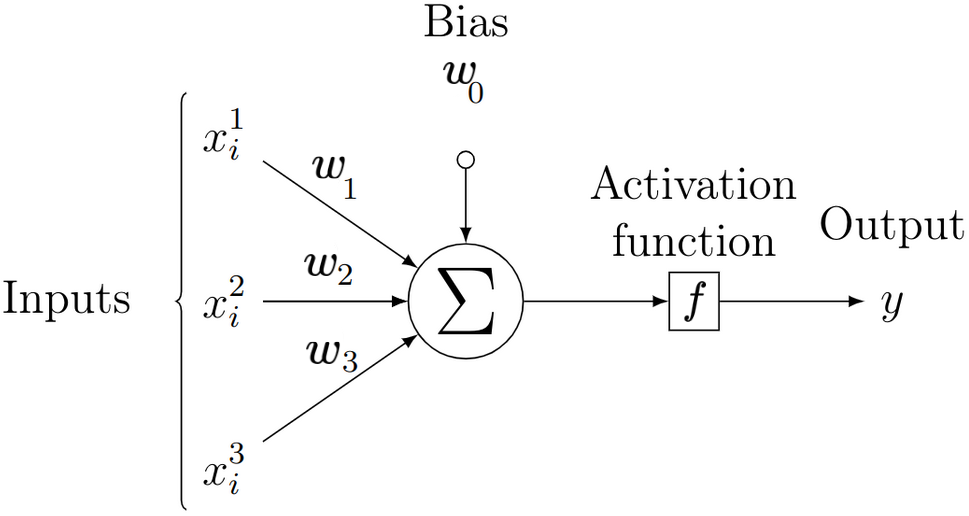
\includegraphics[width=\linewidth]{fig//chap05-stats/perceptron.png}
        \vspace{0.5cm}
        \caption{Visualization of a perceptron with three dimensional inputs $x_{ij}$. Each feature input is multiplied by a weight and everything is summed, along with the bias $w_0$. The result is passed to the activation function $f$, which, in this case, is the Heaviside theta function}
        \label{fig:perceptron}
    \end{figure}
    \end{minipage}
    \hfill
    \begin{minipage}{0.51\linewidth}
    %\vspace{-1.25cm}
        The simplest NN is the Rosenblatt perceptron \cite{Rosenblatt1958TheBrain} (\Fig{fig:perceptron}), an NN with one single neuron that addresses the binary classification problem.\\
        The characteristics of the neuron are:
            \begin{itemize}
                \item The dimension of the input. Each data entry is N-dimensional and each dimension is called a "feature".

                \item Each neuron has N weights, plus one bias, that are tuned through the learning procedure, looking at the data.

                \item The activation function, \ie the function is applied do the dot product $\bm{x}\cdot \bm{w}+w_0$.
                In the case of the perceptron, $f$ is the Heaviside theta function.
            \end{itemize}
    \end{minipage}
    \vspace{0.75cm}
\end{minipage}
\\
Given a set of inputs $\bm{x} \in \mathbb{R}^N$ and a set of weights $\bm{w} \in \mathbb{R}^{N+1}$, the output will be
\begin{equation}
    y=
    \begin{cases}
        1 & \text{if }\sum_{i=1}^N w_i x_i + w_0 >0\\
        0 & \text{Otherwise}
    \end{cases}
\end{equation}
The weights $w_i$ are obtained through the learning procedure.\\
Given $\hat{y}_i$ the truth label of the input $\bm{x}_i$, and $x_{ji}$ the i-th features of the j-th data point:\\
\begin{algorithm}
\caption{Perceptron learning}\label{algo:perceptron}
\begin{algorithmic}[1]
    \State Initialize the weights randomly
    \For{T times} 
        \For{$i=0$ to len($\bm{x}$)}
            \State Compute $y_i(\bm{x}_i)=f(\bm{w}\cdot \bm{x}_i+w_0)$
            \State Update the weights $w_j=w_j+r(\hat{y}_i-y_i)x_{ji}$
        \EndFor
    \EndFor
\end{algorithmic}
\end{algorithm}
\\
Each iteration is called an "epoch". The number of epochs T and the so-called "learning parameter" $r$ are the first two examples of hyperparameters that are chosen by the user.\\
\\
The perceptron is a linear classifier. It means that it can not solve non-linearly separable problems, like an XOR gate, and can not address multiclass classification problems.



\paragraph*{Feedforward neural networks}
Neurons can be connected in layers to build a feed-forward neural network in which each layer is fully connected to the neurons of the previous one.
So, the output of the j-th neuron in the k-th layer is
\begin{equation}
    y^k_{j}=  f^k\left(\sum_i w^k_{ji} y^{k-1}_i + w_{j0}^k\right)
\end{equation}
where $f$ is the so-called activation function of the neuron.\\
The universal approximation theorem \cite{Hornik1989MultilayerApproximators}, asserts that a neural network with one single hidden layer and enough number of neurons can approximate any function.\\
Despite that, it could be needed an arbitrarily large number of neurons to approximate one function using a single layer, so, to simplify the learning process, more layers can be added.\\
A neural network can work in two regimes: evaluation and training.\\
\\
The training regime is the phase in which each weight of the network is tuned learning from the data, and is divided into different steps that will be discussed in detail in the next paragraphs:
\begin{enumerate}
    \item Architecture definition: the number of neurons, layers, and activation functions have to be defined.
    \item Weight initialization: the weights are initialized randomly.
    \item Evaluation of the output: the evaluation phase in which the NN makes the predictions.
    \item Loss evaluation: The loss-function value is computed.
    \item Backpropagation: The gradients of the loss with respect to each weight are computed and the weights are updated.
    \item Iterate from point 3. T times.
\end{enumerate}
After that the NN is trained, it can be used in the evaluation mode, feeding the data to it and collecting the output to obtain the predictions.
\begin{figure}[H]
    %\vspace{-0.cm}
    \centering
    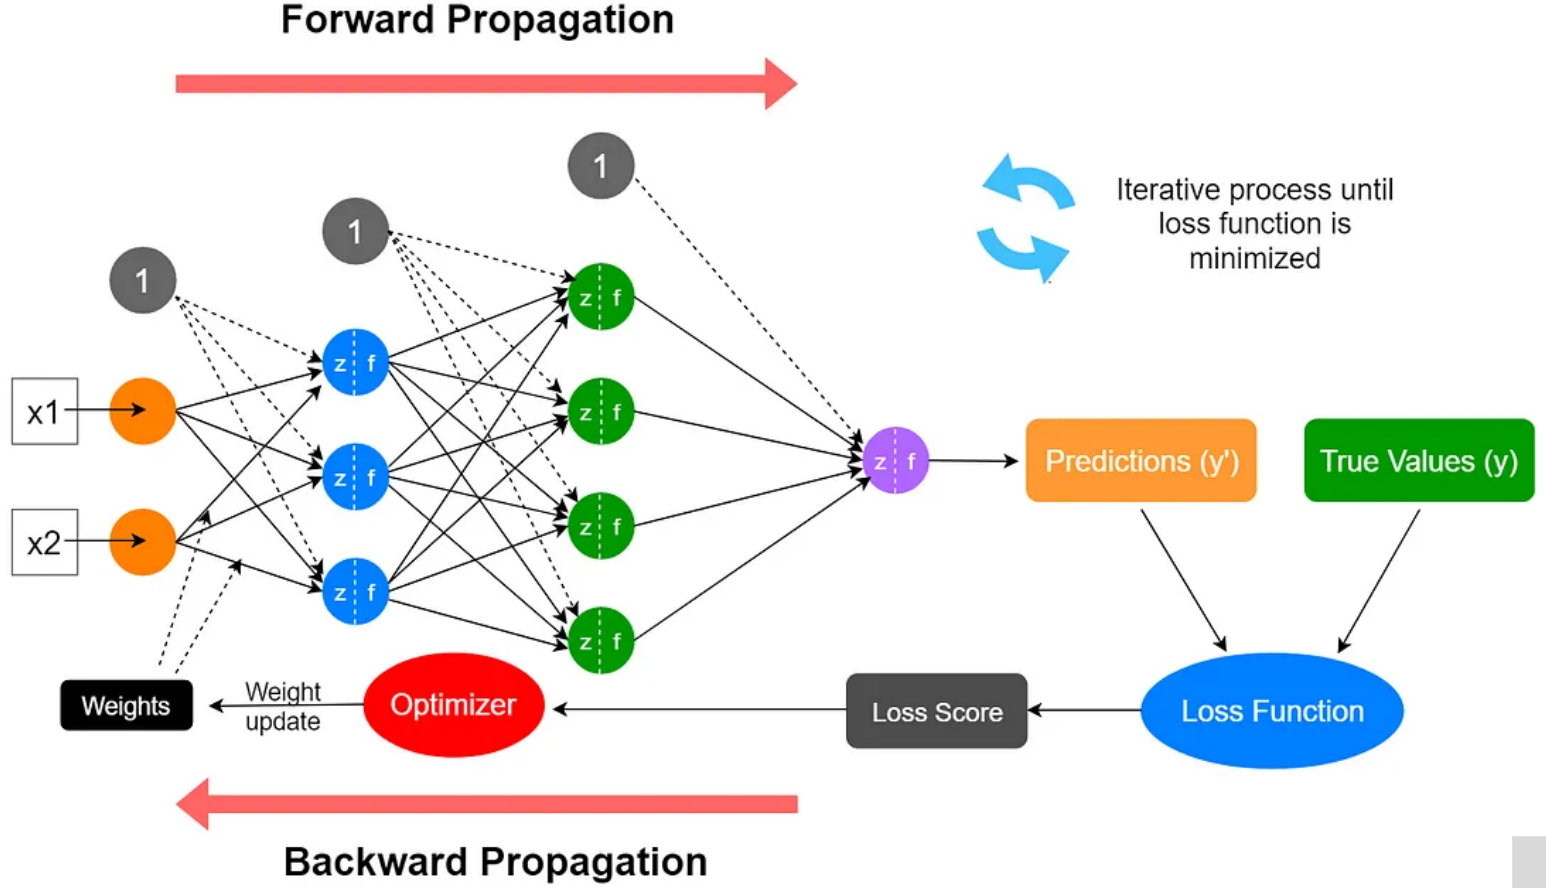
\includegraphics[width=0.85\linewidth]{fig/chap05-stats/dnn.png}
    \caption{Sketch of the training process of a binary classifier NN with 2 input features.}
    \label{fig:dnn}
\end{figure}




\subsection{Loss function}
Under the hood, a neural network is just an optimizer that tries to find the optimal function that minimizes a specific metric.\\
In other words, it is just a tool to perform a multidimensional fit, specifying the objective function in terms of sum and composition of activation function\footnote{This is called "induction bias" and is determined by the architecture of the NN}.\\
The metric that the NN tries to minimize during the learning phase is the so-called "Loss function", a continuous function that compares the prediction of the NN with the labels and has its minimum, ideally, when all the data are predicted correctly.\\
For example, in the case of a regression problem, one of the most used loss functions is the MSE $L=\sum(y_i-\hat{y_i})^2$\footnote{which is the same metric that is minimized when a least squares fit is performed}.\\
\\
In the context of classification problems, the most used loss function is the cross-entropy loss.\\
Assuming that each class belongs to one output neuron, we can use the so-called one-hot encoding, which is a binary representation method where a categorical variable is transformed into a binary vector with a 1 indicating the presence of a particular category and zeros elsewhere\footnote{For example, if we have 3 classes, the 2nd class is represented with the vector [0,1,0]}.\\
The output of the NN will be a vector as long as the total number of classes, and such that the sum of its elements is equal to 1. This can be achieved using the softmax activation function in the output layer (see the paragraph on activation functions).
\\
\\
The one-hot encoding representation is used, instead of the integer encoding that just indexes the classes, to avoid the assumption of natural ordering and to avoid predictions halfway between categories.\\
In the one-hot encoding representation, the cross-entropy loss is
\begin{equation}
    \mathcal{L}=-\sum_i^N w_{\hat{y}_i} \; \bm{\hat{y}_i} \cdot \log \bm{y_i}
\end{equation}
where $\bm{\hat{y_i}}$ and $\bm{y_i}$ are respectively the i-th label and prediction, both in the one-hot encoding representation, while $w_{\hat{y_i}}$ is a weight related to each class that is used to compensate the class imbalance in the training dataset, avoiding the NN to be biased towards one specific class.\\
\\
The cross-entropy loss is related to the likelihood of the multinomial distribution. Assuming m classes, the negative log-likelihood of the multinomial distribution, for a single data point, is\\
\begin{equation}
    -\log \mathcal{L}_{MN_{i}}(\bm{p_i};\bm{n_i})=-\sum_j^m n_j \log p_j + \text{const.}
\end{equation}
where $n_j$ is the number of predicted entries in the j-th class, and $p_j$ is the probability that the data belongs to the j-th class.\\
In the one-hot encoding representation $n_j=\delta_{j\hat{y}_i}$ and $p_j$ is the score ${y}_{\hat{y}_i}$, where $\hat{y}_i$ is the i-th label in the integer representation.
\begin{equation}
    \mathcal{L}_{MN_{i}}=-\bm{\hat{y}_i} \cdot \log \bm{y_i}
\end{equation}
Since each data point is independent from the others, the total log-likelihood is the sum of the single log-likelihoods
\begin{equation}
    \mathcal{L}_{MN}=-\sum_i \bm{\hat{y}_i} \cdot \log \bm{y_i}
\end{equation}

\subsubsection*{Optimizers and backpropagation}
To minimize the loss function, neural networks exploit the technique of gradient descent using different algorithms called "optimizers".\\
The simplest optimizer is the \textit{stochastic gradient descent} (SGD) that, for each data point, computes the gradient of the loss function and updates the weight in the opposite direction of the gradient, propagating it along the network in a procedure called \textit{back-propagation}\footnote{That is just a fancy name to call a composite derivative.}.
\begin{algorithm}
\caption{Stochastic gradient descent}\label{algo:SGD}
\begin{algorithmic}[1]
    \For{i=0 to T}
        \For{j=0 to len($\bm{x}$)}
            \State $\bm{w}=\bm{w}-\eta \grad_{\bm{w}} \mathcal{L}(y_j(\bm{w}),\hat{y}_j)$
        \EndFor
    \EndFor
\end{algorithmic}
\end{algorithm}\\
where $\eta$ is the \textit{learning rate} hyper-parameter.\\
The learning rate should be tuned carefully because a small learning rate will make the NN slow to reach the minimum of the loss, while a huge learning rate will make the gradient descent procedure very  unstable, jumping randomly across the loss hypersurface.\\
\\
To mitigate the fluctuation of the SGD and to improve the computational efficiency, we can compute the gradient on a batch of data and then update the weights
\begin{algorithm}[H]
\caption{Mini-batch stochastic gradient descent}\label{algo:miniSGD}
\begin{algorithmic}[1]
    \For{i=0 to T}
        \For{k=0 to $n_{\text{batch}}$}
            \State $\bm{w}=\bm{w}-\eta \grad_{\bm{w}} \sum_j^{\text{batch size}} \mathcal{L}(y_j^k(\bm{w}),\hat{y}_j^k)$
        \EndFor
    \EndFor
\end{algorithmic}
\end{algorithm}
The gradient is computed and back-propagated using the \textit{automatic differentiation}.
In principle, when the NN is evaluated, a computational graph is built. The nodes of the graphs are just the operators applied to the tensors\footnote{Tensors are just matrices that contain the input data, the weights, and all the intermediate representations of the network.} and, in the backpropagation phase, the gradients of each node are computed and propagated all the way along the graph using the chain rule.\\
Furthermore, NNs perform a lot of simple arithmetic operations that can be performed simultaneously in parallel, so they can be accelerated using graphing processing units (GPU).\\
\\
The list of optimizers is long and each of them has its pros and cons. The SGD has a slower convergence compared to the other optimizers due to its stochastic nature, it is really sensitive to the learning rate, and, especially in high-dimensional and nonconvex problems, it gets stuck very easily in local minima.\\
\\
To address these problems, one of the most used optimizers is ADAM (ADAptive Moment estimator) \cite{Kingma2014Adam:Optimization}. It is able to adapt the learning rate of each parameter individually computing the moving average of gradients and square gradients, ensuring a fast convergence.
\\
The drawback of ADAM is that it has some convergence issues due to its large variance in the first epochs of training in the adaptive learning rate, showing huge fluctuations in the loss, and being too sensitive to the choice of hyperparameters.\\
Trying to stem these issues, recently, a new variant of Adam was proposed: RAdam (Rectified Adam) \cite{Liu2019OnBeyond}.\\
RAdam tries to tackle Adam's convergence issues by introducing a term to rectify the variance of the adaptive learning rate, trying to keep it small in the first epochs.

\begin{figure}[H]
    \centering
    \includegraphics[width=0.85\linewidth]{fig//chap05-stats/radam.png}
    \label{fig:radam}
\end{figure}
As the SGD, all the other optimizers can work on minibatch, evaluating the gradients on a group of data points.
\begin{figure}[H]
    \centering
    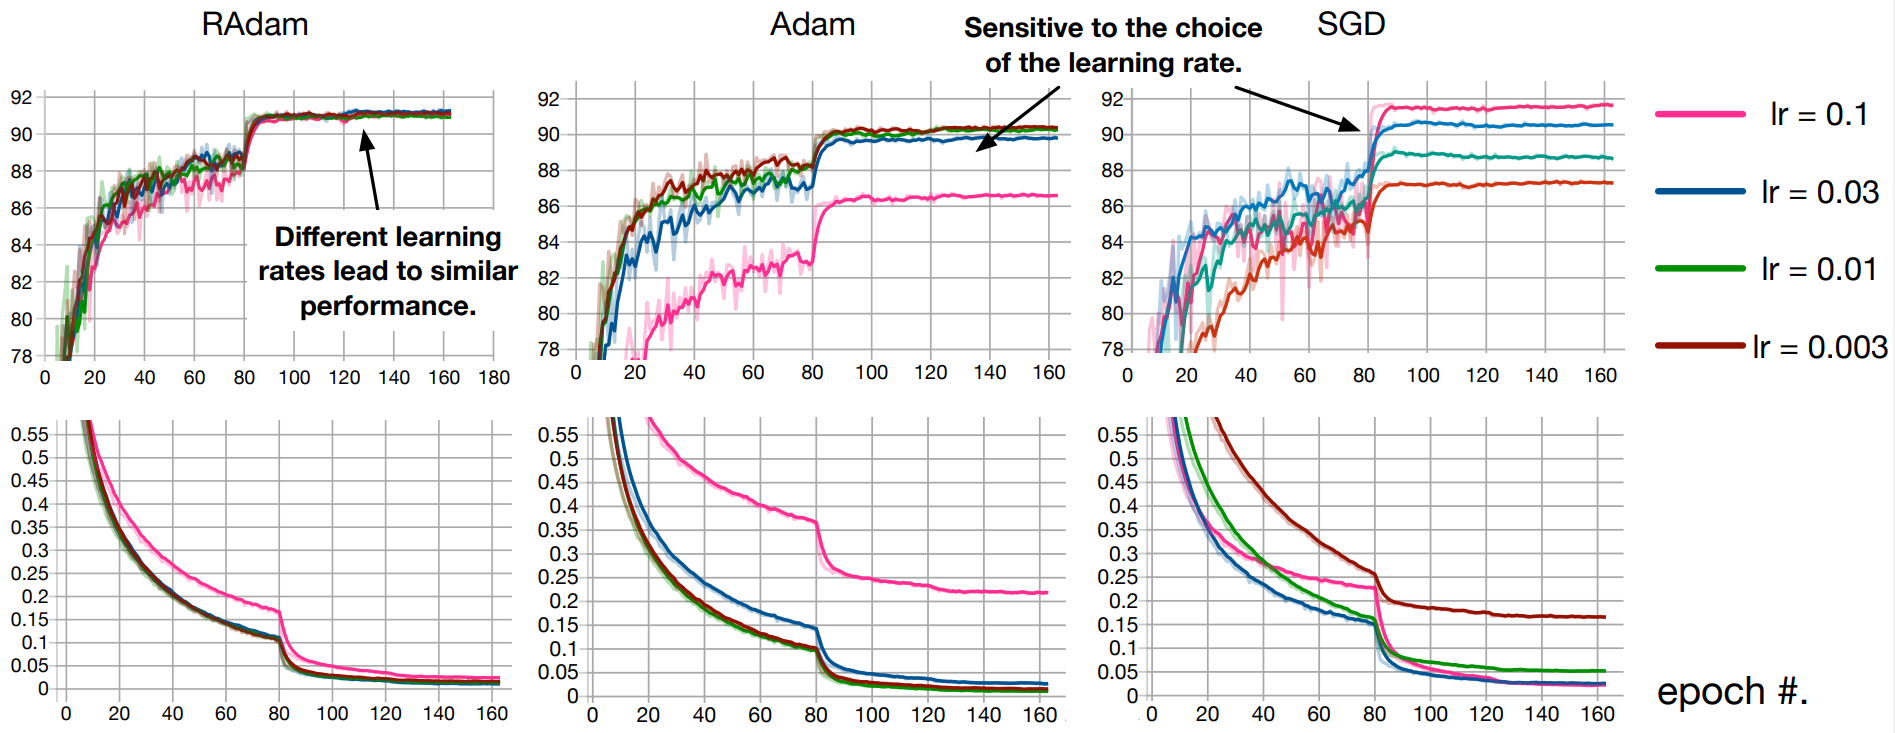
\includegraphics[width=\linewidth]{fig//chap05-stats/radam_loss.png}
    \caption{Evolution in the epochs of the accuracy (top) and loss (bottom) with RAdam, Adam, and SGD with different learning rates on the CIFAR10 problem \cite{Ho-Phuoc2018CIFAR10Humans,Liu2019OnBeyond}.}
    \label{fig:radam_loss}
\end{figure}
\vspace{-1cm}
\subsection{Architecture and complexity}
The architecture of a neural network, specifically the number of layers and neurons, plays a crucial role in determining how well the network can learn and generalize from data.\\
A neural network can be shallow (few layers with many neurons) or deep (many layers with few neurons in each layer). \\
Deep networks tend to capture more complex patterns but suffer the vanishing gradient problem (the magnitude of the gradient decreases propagating back in the network).\\
A high number of neurons improves the capacity to represent functions and makes the network more robust to the noise, embedding the data in a high-dimensional space.\\
Complex NNs are more prone to the \textit{overfitting}.
Overfitting is the behavior of an NN that occurs when the model performs well on the training dataset but doesn't perform in the same way on other data.\\
This occurs because the NN starts to learn the noise and the fluctuations of the training dataset, worsening its generalization capabilities and losing its predictive power.\\
During the training of an NN, overfitting is the most important thing to take under control, and, to do it, the loss is evaluated, for each epoch, not only for the data on which the network is training, but also for other data, called the "validation dataset".
\\
In the case of overfitting, we will see the validation loss that will start to increase, separating from the training loss.\\
On the other hand, if the network is too simple, we will fall into the underfitting, \ie the objective function represented by the NN is too simple to fit the data.
\vspace{-0.15cm}
\begin{figure}[H]
    \centering
    \includegraphics[width=1\linewidth]{fig/chap05-stats/overfit.jpg}
    \caption{Representation of underfitting, of a good fit, and of overfitting. The right plot shows the behavior of the validation loss in case of overfitting}
    \label{fig:overfitting}
\end{figure}
Several techniques can be used to prevent the overfitting:
\begin{itemize}
    \item Diminish the number of neurons and the complexity of the network
    \item Increase the size of the training dataset
    \item Add a penalty term to the loss function, like the L2 regularization
    \begin{equation}
        \mathcal{L}^{'}=\mathcal{L}+\lambda \sum ||\bm{w}||^2
    \end{equation}
    a term that penalizes scenarios in which the weights assume large values (that usually is one consequence of the overfitting)
    \item \textbf{Early stopping}: stop the learning when the validation loss starts to separate from the training loss.
    \item \textbf{Dropout}: the dropout \cite{Srivastava2014Dropout:Overfitting} is the probability that, in a single epoch during the training, one neuron will just be ignored and its connection with the rest of the network will be dropped out. \\
    By randomly disabling neurons, dropout prevents any single neuron from becoming overly specialized on a specific feature of the training data.\\
    Furthermore, introducing this stochastic behavior can also accelerate the training, preventing the network from getting stuck in local minima of the loss.\\
    The dropout rate is another hyperparameter that should be tuned carefully by the user.
\end{itemize}

\paragraph*{Residuals}\hspace{1cm}\\

\begin{minipage}{\linewidth}
    \vspace{0.1cm}
    \begin{minipage}{0.55\linewidth}
        To mitigate the effect of the vanishing gradient, some "skip connections" can be used to back-propagate the gradients better through the network, ensuring that the output of a layer is added together with the output of a later layer.\\
        If the dimensionality at the beginning of the connection is different from the dimensionality at the end of the connection, the residual can be multiplied by a linear projection to align the dimensions.\\
        These networks are called "residual networks" or ResNets \cite{He2015DeepRecognition}.
    \end{minipage}
    \hfill
    \begin{minipage}{0.4\linewidth}
        \centering
        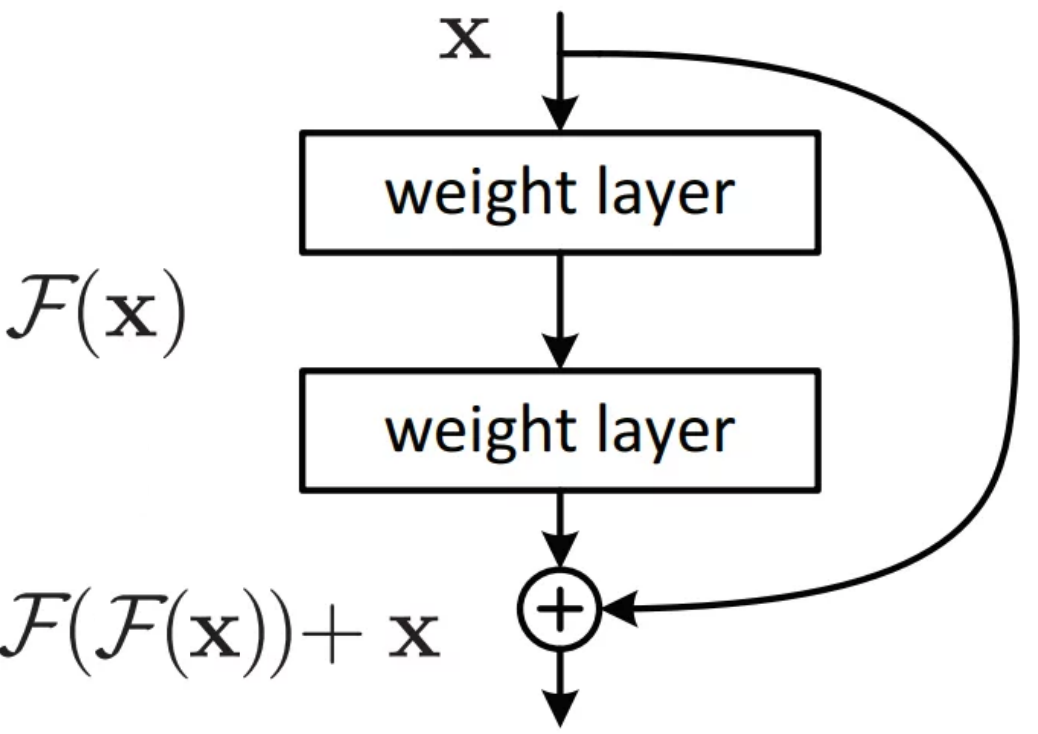
\includegraphics[width=1\linewidth]{fig/chap05-stats/res.png}
        \captionof{figure}{Visualization of the skip connection in a residual block of a ResNet.}
        \label{fig:resnet}
    \end{minipage}
\end{minipage}


\subsubsection*{Activation functions}
The activation functions in a neural network must possess some properties:
\begin{itemize}
    \item Continuity and differentiability: to compute the gradients of the loss with respect to the weights.
    \item Non-linearity: the activation functions must be non-linear because the composition of linear functions is still a linear function
    \item Their derivative must be bounded to avoid the so-called "explosive gradient", the opposite phenomena of the vanishing gradient.
\end{itemize}
The activation functions of the output layer are different from the others.\\
In a regression problem, the activation function of the output layer is linear, while, in the case of classification, using the one-hot encoding, the used activation function is the \textit{softmax} function
\begin{equation}
    {\textit{softmax} (\mathbf {x} )_{j}={\frac {e^{x_{j}}}{\sum _{k=1}^{K}e^{x_{k}}}}} \quad \text{for } j=1,\dots,K
\end{equation}
where K is the number of classes.\\
The softmax function ensures that the output of the network is a vector of length K, such that the sum of its elements is always 1. This allows us to treat the output of the network as a probability.\\
\\
In the hidden layers, instead, we have more choices. The first activation functions ever used were the logistic function and the hyperbolic tangent, which are related to each other, and have a finite codomain.\\
These two functions were chosen due to the interpretation that we can give to them, like in the perceptron\footnote{in fact the logistic function can be seen as the "smoothed version" of the Heaviside theta function}: when the function is around its lower bound, the neuron is off, and when the function is around its upper bound, the neuron is on.
\begin{align}
    \tanh(x)&= \frac{e^x-e^{-x}}{e^x+e^{-x}}=2\sigma(2x)-1  \\
    \sigma(x)&=\frac{1}{1+e^{-x}} 
\end{align}
But the derivative of these functions is significantly different from zero just in a narrow range, slowing the learning of the network once the function saturates.\\
\\
Another activation function that was proposed was the ReLU (Rectified linear unit)\cite{FredAgarap2018DeepReLU}, one of the most used activation function
\begin{equation}
    \textit{ReLU}(x)=\max(0,x)
\end{equation}
The ReLU allows a better propagation of the gradients and is very efficient from the computational point of view since is a piecewise linear function and the gradient is a constant.\\
Furthermore, the ReLU introduces a sparse representation in the network:
when the network is initialized, only about half of the neurons have a non-zero output, and this has a regularization effect similar to the dropout.\\
Despite that, the ReLU suffers the so-called "dying ReLU problem": some units can be pushed into some states in which they become inactive to all possible inputs, making an always zero gradient. In this state, the neuron enters an endless dead state.\\
\\
To solve the dying ReLU problem, a lot of ReLU-like functions were proposed. In this work, the used activations function was the recently proposed Swish \cite{Ramachandran2017SearchingFunctions}. 
\begin{equation}
    \textit{Swish}(x; \beta)=\frac{x}{1+e^{-\beta x}}
\end{equation}
where $\beta$ is a learnable parameter.\\
The Swish function has a smooth gradient that can avoid the dying ReLU problem, ensuring the neurons continue to produce non-zero outputs.

\begin{figure}[H]
    \centering
    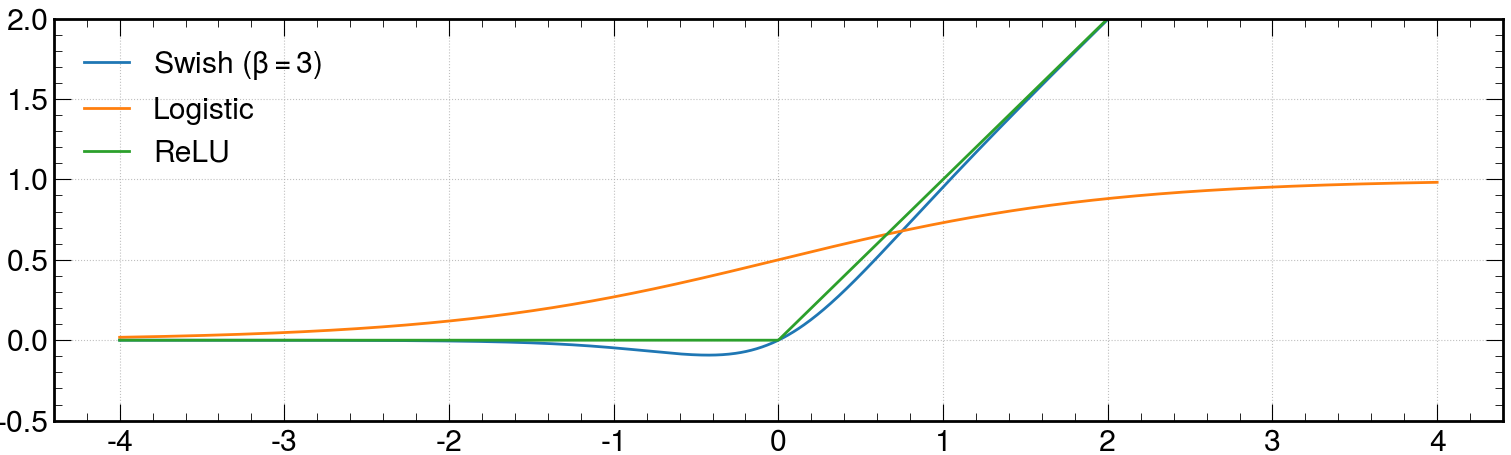
\includegraphics[width=0.85\linewidth]{fig//chap05-stats/act.png}
    \caption{Logistic, ReLU, and Swish activation functions.}
    \label{fig:activation}
\end{figure}

Anyway, despite all the motivations that were provided, the best activation function does not exist and, in general, in the field of neural networks, every choice is justifiable only through heuristics.


\subsubsection*{Input normalization}
The features of the input data have different distributions with different ranges and scales. The parameters associated with each feature will also have different scales and this can lead to a loss function whose gradient will be biased toward certain parameters, as shown in \Fig{fig:loss_normalization}.\\
\vspace{-0.5cm}
\begin{figure}[H]
    \hspace{-0.5cm}
    \centering
    \includegraphics[width=0.85\linewidth]{fig/chap05-stats/loss_norm.png}
    \vspace{0.5cm}
    \caption{Loss curve levels in case of non-normalized inputs (left) and normalized inputs (right) \cite{NormalizingNormalization.}.}
    \label{fig:loss_normalization}
    \vspace{-0.5cm}
\end{figure}
To make the learning of the network more stable and faster, we can normalize all inputs to a standard scale, allowing us to use larger learning rates.\\
Furthermore, this also avoids the saturation of a large number of activation functions in the first epochs which can lead to a slow learning due to the small gradients in the saturation regime.\\
For specific activation functions, like the ReLU-like, having inputs with zero mean will cause $\sim 50\%$ of the neurons to be inactive, creating a sparse representation (see paragraph on activation functions).\\
\\
One of the most used input normalization techniques is the \textit{Batch norm} \cite{Ioffe2015BatchShift}, which consists of normalizing each input feature with its mean and standard deviation computed across all the batch
\begin{equation}
    \bm{x}_i^{'}=\frac{\bm{x}_i-\mu_i}{\sigma_i+\epsilon}
\end{equation}
where $\bm{x}_i$ is the i-th feature of the input tensor and $\epsilon$ a small number added to prevent numerical issues.\\
\\
Despite that,  the mean and the standard deviations are not robust estimators, and, if a feature has significant outliers, the batch norm can create distributions not centered around zero.\\
To overcome this issue, we can replace the mean and the standard deviation with more robust estimators like the median, we can just clip the outlier to a threshold value, or we can apply a function that will shrink them.\\
In this work, the applied normalization to positive value features that have significant outliers is the following
\begin{equation}
    \bm{x}_i^{'}=\frac{\log \left(1+\bm{x}_i \right)-\mu_{i}^{\log}}{\sigma_i^{\log}+\epsilon}
\end{equation}
where $\mu_i^{\log}$ and $\sigma_i^{\log}$ are the mean and the standard deviation computed on $\log(1+\bm{x}_i)$

\paragraph*{Internal normalization}
During the training, the distribution of each layer’s weights changes, as the parameters of the previous layers change.
This slows down the training by requiring lower learning
rates. \\
This behavior is called "internal covariate
shift", and we can address the problem by introducing a normalizing layer in the network.\\
\\
We could use the batch norm or, instead, the layer norm \cite{Ba2016LayerNormalization}, which is the same thing as the batch norm but the mean and the standard deviation are computed across the features instead of across the batch.\\
In some architectures (like RNN) or domains (natural language processing), the layer norm was proven to work better than the batch norm.



\subsubsection*{Weight initialization}
The initialization of the weights is strictly related to the chosen normalization and the chosen activation functions.\\
Large or small initialization values will lead respectively to the problem of exploding and vanishing gradient.\\
An appropriate initialization should impose a zero mean of the weights and a variance that should stay constant across all the layers.
\\
To do it, if we use activation functions that are linear around zero (like the $\tanh$), we can use the Xavier initialization \cite{Glorot2010UnderstandingNetworks}.
\begin{equation}
    W\sim U \left[-\frac{\sqrt{6}}{\sqrt{n_j+n_{j+1}}},\frac{\sqrt{6}}{\sqrt{n_j+n_{j+1}}} \right]
\end{equation}
where $n_j$ is the number of units in the j-th layer.\\
If we use ReLU-like functions, instead, we should use the He initialization \cite{he2015delving}.
\begin{equation}
    W\sim \mathcal{N}\left(0,\frac{2}{n^l}\right)
\end{equation}
the derivation of these two distributions is simple and is provided in the respective papers, and consists only of imposing the variance of the output of a unit to be constant across all layers.

\subsubsection*{Hyperparameter optimization}
In this section, we have introduced many hyperparameters like the learning rate, the size of the network, etc. These parameters have to be tuned to obtain the best performances.\\
\\
The simplest way to perform a hyperparameters search is to perform a \textit{grid seach}, which consists of creating a grid of parameters and repeating the training for each combination of them.\\
However, this simple algorithm is feasible only for small networks because the number of trainings required depends on a combinatorial factor.\\
\\
Clever ways to find the optimal set of hyperparameters can involve Bayesian optimization methods, but, if the model is too big and the time and the computing resources are very scarce, the only remaining tool is manual optimization in which the user tries to find a good set of hyperparameters by trying with just a couple of trainings.


\subsection{Attention mechanism}
Attention is a mechanism that enables models to focus on specific parts or elements of the input data while performing a task. It is particularly important in fields like natural language processing (NLP) and computer vision.\\
Attention networks belong to the class of sequence-to-sequence (seq2seq) models. 
One of the most common seq2seq tasks is the language translation in which the model takes as input one sentence (\ie a sequence) in a language and translates it into another language (\ie another sequence).
This means that the inputs of the network are 3 dimensional: one is the batch dimension, one is the sequence dimension, and the last is the feature dimension.\\
In particle physics, seq2seq models enable us to treat each event as a sequence composed of its particles and to maintain the event structure.

\subsubsection*{Scaled dot product}
One particular method to implement the attention is the "scaled dot product" \cite{Vaswani2017AttentionNeed}.\\
\begin{equation}
    \textit{Attention}(Q,K,V)=\textit{Softmax}\left(\frac{QK^T}{\sqrt{d_k}}\right)V
\end{equation}
\vspace{0.2cm}\\
The scaled dot product has 3 inputs \cite{Vaswani2017AttentionNeed}: the "Query" (Q) of dimensions $(N, S_2, d_k)$ and "Key" (K) of dimension $(N, S_1, d_k)$, and the "Value" (V) of dimension $(N, S_2, d_k)$, where $N$ is the batch size, $S_1,S_2$ the length of the sequences and $d_k$ the number of neurons of the previous layer in the network.\\


\begin{minipage}{\linewidth}
    \begin{minipage}{0.53\linewidth}
        $Q,K,V$ are linear embeddings of the layer inputs, so $Q,K,V=W_{Q,K,V} \cdot X_{Q,K,V}$ where $W$ are the weights learned during the training.\\
        \\
        The $\textit{Softmax}\left(\frac{QK^T}{\sqrt{d_k}}\right)$ is the matrix of the "Attention-scores" and has dimension $(N,S_2,S_1)$, so it exploits the dot product between the Query and Key tensors to compute and assign a score to all the pairs in the two sequences, performing a weighted average on the Value tensor.\\
    \end{minipage}
    \hfill
    \begin{minipage}{0.43\linewidth}
        \vspace{-0.7cm}
        \centering
        \includegraphics[width=0.5\linewidth]{fig//chap05-stats/translation.png}
        \vspace{0.6cm}
        \captionof{figure}{Attention scores between sentences in English and French. The network has learned to recognize which words have the same meaning also if they are in a different order.}
        \label{fig:Translation}
    \end{minipage}
\end{minipage}
\vspace{0.1cm}\\
The inputs of the scaled dot product are called Key, Query, and Value as an analogy to the search engine systems: a search engine will compare the user Query with the Key associated with all the pages available in the database and will return the Value, \ie the page, which associated key best match the Query.  
\\
Attention networks are a rare example of explainability. By studying attention scores we can understand what the network is learning. Usually, instead, neural networks are black boxes that tend to learn representations that are difficult to understand by humans.
\\
\\
In particle physics, this approach is particularly feasible for two reasons
\begin{itemize}
    \item There is a natural way to handle arrays of different lengths: we can just fix the maximum length of the sequence and, for the absent particles, just impose the respective attention scores to zero.\\
    This allows us to maintain the ragged structure of the event.
    \item Attention networks are invariant for permutation of the elements in the sequence, so we are not forced to introduce an ordering between the particles
\end{itemize}


\paragraph*{Multihead attention}
One set of $W_Q,W_K,W_V$ matrices is called an \textit{attention head}, but we can stack multiple attention heads together, allowing the model to learn different representations of the sequence separately.\\
The different heads can be computed in parallel and their output, at the end, is concatenated.

\begin{figure}[h!]
    \centering
    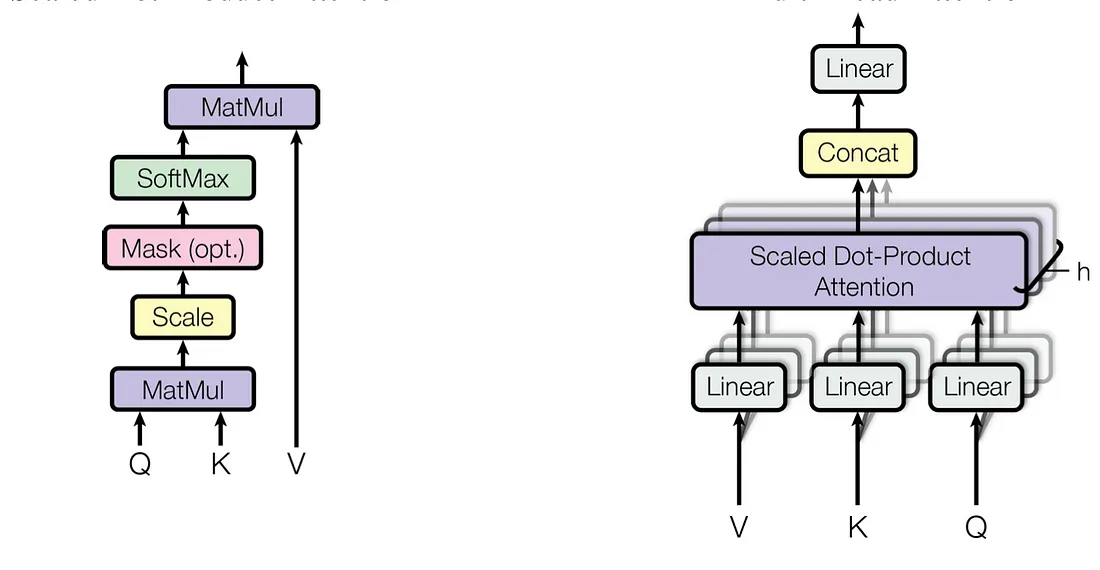
\includegraphics[width=0.75\linewidth]{fig//chap05-stats/multihead_attention.png}
    \caption{(Left) scaled dot product, (right) multi-head attention \cite{Vaswani2017AttentionNeed}.}
    \label{fig:multihead}
\end{figure}

\paragraph*{Self-attention} With a "self-attention layer" we refer to a scaled dot product layer in which $Q,K,V$ are linear embeddings of the same input $\bm{X}$.\\
It enables the model to capture contextual information and relationships between elements in the sequence, computing attention scores for each element with respect to all the others.\\
These attention scores determine how much each element should focus on the others and the resulting weighted sum provides a contextually enriched representation of the sequence.

\paragraph*{Cross-attention}
Cross-attention is an extension of the self-attention mechanism that allows a model to attend to elements in a target sequence based on the elements in another sequence (called context sequence).\\
The Key and Value vectors are linear embeddings of the context sequence while the Query is a linear embedding of the target sequence.\\
Cross-attention allows models to establish relationships between elements in different sequences, also of different lengths, making it suitable for tasks that involve aligning information from one sequence with another.

\paragraph*{Self-attention pooling}


Pooling is a technique used to downsample or reduce the dimensionality of feature maps, or in our case a sequence, retaining important information.\\
As already discussed, we are interested in classifying an event as a signal or background, so we have to reduce the dimensionality of the sequences that contain all the particles in the events, to just one.\\
Self-attention pooling \cite{Safari2020Self-attentionRecognition} is a pooling layer inspired by self-attention
\begin{equation}
    \textit{Self-Att. Pool}=\textit{Softmax}(\bm{W} \bm{X}^T)\bm{X}
\end{equation}
where $\bm{X}$ is the input tensor of size $(N,S,F)$ and $\bm{W}$ is a set of trainable weight of size $(S^{'},F)$, where $S^{'}$ is the target size of the output sequence.\\
Therefore, self-attention pooling is a weighted average of the sequence features where the weights are the attention scores learned by the self-attention mechanism.













%%%%%%%%%%%%%%%%%%%%%%%%%%%%%%%%%%%%%%%%%%%%%%%%%%%%%%%%%%%%%%%%%%%%%%%%%%%%%%%
%%%%%%%%%%%%%%%%%%%%%%%%%%%%%%%%%%%%%%%%%%%%%%%%%%%%%%%%%%%%%%%%%%%%%%%%%%%%%%%
%%%%%%%%%%%%%%%%%%%%%%%%%%%%%%%%%%%%%%%%%%%%%%%%%%%%%%%%%%%%%%%%%%%%%%%%%%%%%%%
%%%%%%%%%%%%%%%%%%%%%%%%%%%%%%%%%%%%%%%%%%%%%%%%%%%%%%%%%%%%%%%%%%%%%%%%%%%%%%%

\section{Signal extraction}
\subsection{Likelihood construction}
The signal extraction procedure relies on a maximum likelihood fit of a binned distribution of one or more observables.\\
The likelihood is constructed as the product of Poisson distributions, one for each bin, that contains the parameter of interest (POI) to fit.\\
Given $C$ channels\footnote{A channel is defined by a set of cuts and selections that have the scope to isolate the signal and reject the background or viceversa}, each that contains $P_c$ processes, represented with histograms with $B_c$ bins, once we have the signal and the background MC predictions $s_{cb}$, $b_{cb}$, and the observed bin content $n_{cb}$, the likelihood is \cite{Khachatryan2015PreciseTeV}
\begin{equation}
    \mathcal{L}(\mu)=\prod_c^C \prod_b^{B_c} \frac{(\mu s_{cb}+b_{cb})^{n_{cb}}}{n_{cb}!} e^{-(\mu s_{cb}+b_{cb})}
\end{equation}
where index $c$ stands for "channel", $p$ for "process", $b$ for "bin"
In this case, the POI is the signal strength $\mu$, which is estimated by finding the value that maximizes the likelihood. The optimization problem is solved using the \textsc{MIGRAD} algorithm \cite{James1998MINUIT:Manual}, implemented in the \textsc{MINUIT2} library, that performs a line search in the direction of the gradient and updates the covariance matrix (inverse of the Hessian matrix) with each step.\\
To improve the numerical stability, the software implementation exploits the negative log-likelihood $\textit{NLL}=-\log{\mathcal{L}}$ instead of the likelihood in the form of the \Eq{eq:likelihood}  
\begin{equation*}
    \hat{\mu}=argmin_\mu - \log{\mathcal{L}(\mu)}
\end{equation*}
The predictions for each process are obtained through MC simulations, that are rescaled to match the total number of expected observed events. If $N^{MC}_{cp}$ is the total number of entries in the histogram relative to the process $p$ in the channel $c$, the respective entries have to be rescaled by a factor $w_{cp}$
\begin{equation}
    w_{cp}=\frac{\mathcal{L_I} \sigma_p \epsilon_{cp}}{N_{cp}}
\end{equation}
where $\mathcal{L_I}$ is the integrated luminosity, $\sigma_p$ the cross-section of the process $p$ and $\epsilon_{cp}$ the fraction of events of the process $p$ that pass the preselection defined by the channel $c$ that is estimated using MC events. 
\\
\newpage
\subsubsection*{Systematic uncertainties}
To incorporate in the model all the relevant uncertainties (\ie luminosity and rate uncertainties, uncertainties related to the detector resolution, etc.) we add to the likelihood the so-called nuisance parameters $\vec{\theta}$.\\
The likelihood becomes \cite{Conway2011IncorporatingSpectra}
\begin{equation}\label{eq:likelihood}
    \mathcal{L}(\mu,\vec{\theta})=\prod_c^C \prod_b^{B_c} Poiss \big( n_{cb}| \lambda_{cb}(\mu,\vec{\theta}) \big)  \prod_k  \pi_{k}(\theta_k)
\end{equation}
where $\pi_{k}$ is the prior probability distribution of the nuisance $\theta_k$.\\
The expectation value $\lambda_{cb}$ of the Poisson distribution now depends on the nuisance parameters that can be classified into normalization nuisances, shape nuisances, and statistical nuisances.
\begin{equation}\label{eq:lambda}
     \lambda_{cb}( \mu,\vec{\theta})=\sum_p^{P_c}M_{cp}(\mu) N_{cp}(\vec{\theta}_n)y_{cpb}(\vec{\theta}_s)+E_{cb}(\vec{\theta}_{MC})
\end{equation}
The term $M_{cp}(\vec{\mu})$ is the physical model that contains the POI to fit, $N_{cp}(\vec{\theta_n})$ contains the factors relative to normalization nuisances, $y_{cpb}(\vec{\theta}_s)$ is the predicted content of each bin (that depends on shape nuisance parameters) and $E_{cpb}(\vec{\theta}_{MC})$ represents bin per bin the statistical error of the Monte Carlo predictions.\\
In the absence of systematic uncertainties, we have $N_{cp}=1$ and $E_{cb}=0 \quad \forall c,p,b$ and
$M_{cp}=\mu$ if $p$ is a signal process, otherwise $M_{cp}=1$; while $y_{cpb}$ is just the predicted bin content for each process.\\
All the nuisance parameters $\theta_k$ are defined in units of standard deviations\footnote{it means that $\theta=\pm 1$ correspond to a 68\% CL interval.}.\\
Given that we know the central values and the standard deviations of all the variations, following the maximum entropy principle \cite{Jaynes2003ProbabilityScience}, we can use the normal distribution as a prior for all the nuisance parameters.
\begin{equation}
    \pi_k(\theta_k)=\mathcal{N}\left(\theta_k|0,1\right)=\frac{1}{\sqrt{2\pi}}e^{-\theta_k^2/2}
\end{equation}
\begin{itemize}
    \item \textbf{Normalization nuisances} are multiplicative corrections that affect the normalization of one process (\eg the cross-section uncertainties) or of all processes (\eg the luminosity uncertainties).\\
    This type of uncertainty does not change the shape of the histogram but changes the number of expected events.\\
    In $\lambda_{cb}$ [eq. \ref{eq:lambda}], they are represented by the term
    \begin{equation}
        N_{cp}\left(\vec{\theta}_n\right)=k_{cp}^{\theta^{(n)}_k}
    \end{equation}
    where $k_{cp}$ the relative $+1 \sigma$ variation from the nominal event yield for the process $p$ in the channel $c$ estimated through theory calculation of external measurements, while $\theta_{k}$ is the relative normalization nuisance parameter.\\
    \newpage
    \item \textbf{Shape nuisances}: Shape-changing nuisances are produced by uncertainties
    that cause a different variation of event yields for each different bin.\\
    The model parameters are varied of $\pm 1 \sigma$ around their central value, creating an “Up” and a “Down” variation.\\
    The bin content $y_{cpb}$ has to be modified by multiplying a continuous and differentiable function of $\vec{\theta}_{s}$, so, given $\delta_b^\pm$ the differences between the $\pm 1 \sigma$ bin content variations of the bin and the nominal one, the up and down variations are interpolated with a spline in a procedure called "vertical morphing" \cite{Conway2011IncorporatingSpectra}
    \begin{equation}
    f_b\left(\theta_k^{(s)}\right)=
        \begin{cases}
            {\frac{1}{2}}\left((\delta_b^{+}-\delta_b^{-})\theta_k+{\frac{1}{8}}(\delta_b^{+}+\delta_b^{-})(3\theta_k^{6}-10\theta_k^{4}+15\theta_k^{2})\right) & \text{for } |\theta_k|\leq 1\\
            \theta_k \delta^+ & \text{for } \theta_k>1\\
            -\theta_k \delta^{-} & \text{for } \theta_k<-1
        \end{cases}
    \end{equation}
    The term $y_{cpb}(\vec{\theta}_s)$ is then defined as 
    \begin{equation}
        y_{cpb}(\theta_s)=max\left(0,y_{cpb}+\sum_k f_{cpb}\left(\theta_k^{(s)} \right)\right)
    \end{equation}
    In this way, we can clip $y_{cpb}$ to 0 preventing the height of the bin from being negative.\\
    The vertical morphing procedure is shown and described in detail in \Fig{fig:morphing}



    
    \item \textbf{MC statistical nuisances}: The MC events used to predict the expected signal and background yield in each bin are limited.\\
    To model the statistical MC uncertainties, we could add a nuisance parameter per bin per process, following the Barlow-Beeston approach \cite{Barlow1993FittingSamples}.\\
    But, if we have enough statistics in each bin, we can just use a nuisance parameter per bin that scales the sum of the processes yield, following the Barlow-Beeston lite approach \cite{Barlow1993FittingSamples}.\\
    The term $E_{cb}$ in $\lambda_{bc}$ is the term related to the statistical uncertainties is
    \begin{equation}
        E_{cb}(\vec{\theta}_{MC})=\theta_b\left(\sum_p \left(e_{cpb}N_{cp}(\vec{\theta}_n)M_{cp}(\mu)\right)^2 \right)^{1/2}
    \end{equation}
    where $N_{cp}$ and $M_{cp}$ are the normalization factor and the physical model defined before.
    $e_{cpb}$ is the Poissonian standard deviation of the b-th bin in the process p. Considering that the $\hat{\sigma}_{Poiss}=\sqrt{y_b}$ and that the bin height has to be rescaled to match the expected number of observed events, $e_{cpb}$ is
    \begin{equation}
        e_{cpb}=w_{cp} \sqrt{N_{cpb}^{MC}}   =\frac{\mathcal{L_I} \sigma_p \epsilon_{cp}}{N^{MC}_{cp}} \sqrt{N^{MC}_{cpb}}
    \end{equation}
    where $N_{cpb}$ is the number of MC events in the b-th bin.\\
    The term $E_{cb}$ scales, linearly with the nuisance parameter, the event yield of the bin with the root square sum of the Poisson uncertainties of each process.\\
\end{itemize}
\begin{figure}[h!]
    \centering
    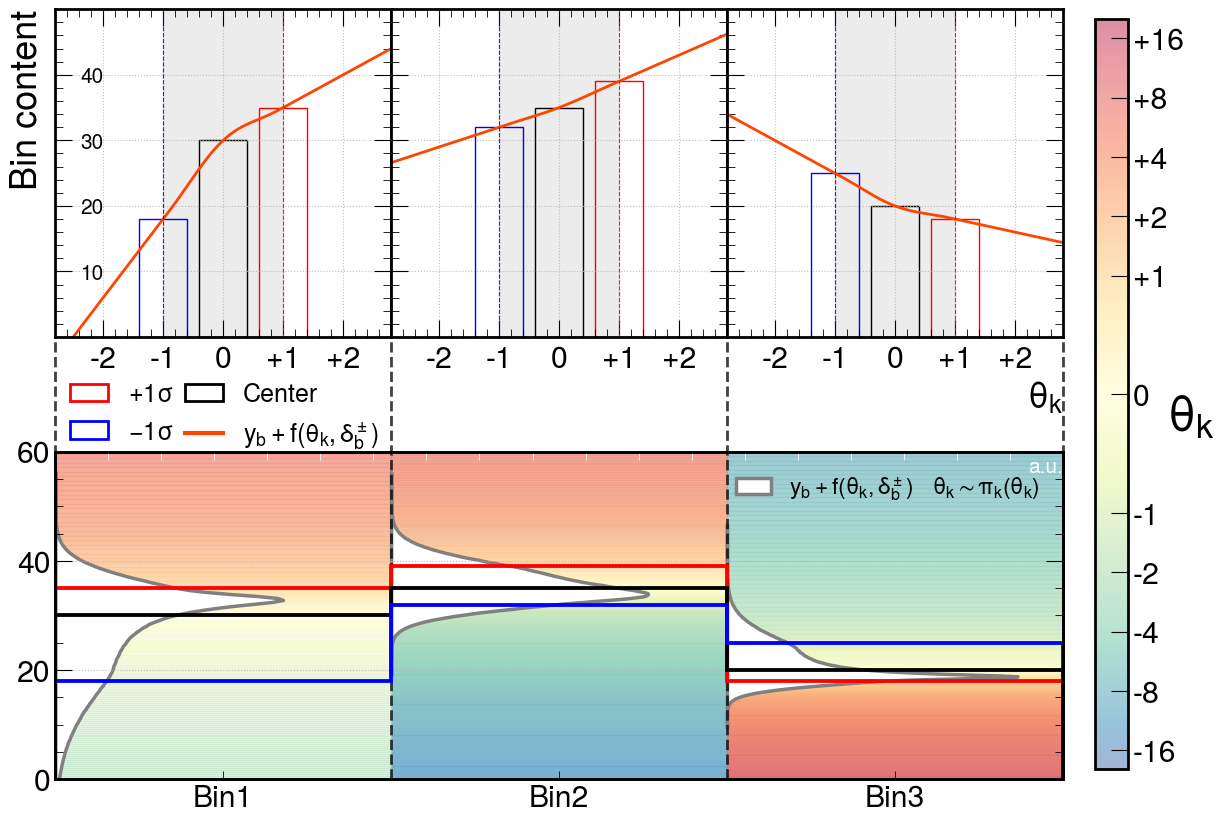
\includegraphics[width=\linewidth]{fig//chap05-stats/morphing.png}
    \caption{In the lower panel is represented an example of a histogram with 3 bins. The black line represents the histogram, the blue and the red lines represent the $\pm 1 \sigma$ shape variations.
    In the top panel, each bin is represented with its $\pm 1 \sigma$ variations and, on top of them, the $y_b+f(\theta_k,\delta_b^\pm)$ interpolation is shown with a red line. In the background of the lower panel, a color map shows, for each value of the bin height, the corresponding value of the nuisance parameter $\theta_k$, while the rotated vertical white shadow represents, for each bin, the probability distribution in arbitrary units of the expectation value of the Poisson distribution $\lambda_b=y_b+f(\theta_k,\delta_b^\pm)$ drawing $\theta_k$ from the normal prior.}
    \label{fig:morphing}
\end{figure}
\newpage
\vspace{0.5cm}
\paragraph*{Smoothing}
For some systematics, up and down variations can lead to significant statistical fluctuations in the less populated bins due to low MC statistics, which, usually, are the high signal purity regions of the background histogram.\\
To overcome this inconvenience, a smoothing procedure is applied.

\begin{algorithm}[H]
\caption{Smoothing algorithm}\label{algo:smooth}
\begin{algorithmic}[1]
    \State Compute $r^{up}_b=y_{b}^{up}/y_b$ and $r^{down}_b=y_{b}^{down}/y_b$
    \State Compute $\delta r_b=\left(r^{up}_b-r^{down}_b\right)/2$
    \State Define $\hat{r}^{up}_b=1+\delta r_b$ and $\hat{r}^{down}_b=1+\delta r_b$
    \State Given $x_b$ is the position of the bin centers, apply the LOWESS smoothing algorithm to the points $(x_b,\hat{r}^{up}_b)$ and $(x_b,\hat{r}^{down}_b)$, finding the functions $f^{up}(x)$ and $f^{down}(x)$
    \State Redefine $y_b^{up}=y_b f^{up}(x_b)$ and $y_b^{down}=y_b f^{down}(x_b)$
\end{algorithmic}
\end{algorithm}
The LOWESS algorithm \cite{Cleveland1979RobustScatterplots} (LOcally WEighted Scatterplot Smoothing) performs different linear regressions on a sliding window iteratively, weighting each point accordingly with its distance from the fitted line in each window.

\iffalse
\begin{algorithm}[H]
\caption{LOWESS algorithm}\label{algo:LOWESS}
\begin{algorithmic}[1]

    \State For each point $(x_i,y_i)$, create a window of a fixed length L.
    \State Define the weights $w_{1,ij}(x)=(1-|(x_j-x_i)/L|^3)^3 \; \Theta(L-|x_j-x_i|)$ where $\Theta$ is the Heaviside theta function.
    \State Perform a linear regression in each window, weighting each point with the defined weights $w_{1,ij}$. 
    \State Define $\hat{y}_i=f_{1,i}(x_i)$ where $f_{1,i}$ is the linear function obtained from the linear regression in each window.
    \State Compute the residuals $s_i=|y_i-\hat{y}_i|$.
    \State Normalize the residuals with $s_i=s_i/(6 m(s_i))$ where $m(s_i)$ is the median of the residuals.
    \State Define the weights $w_{2,i}=(1-s_i^2)^2 \; \Theta(1-s_i)$ 
    \State Perform a second linear regression on the points $(x_i,\hat{y}_i)$ weighting each point in the window with $w_{2,i}$, obtaining the functions $f_{2,i}$
    \State The smoothed curve is $(x_i,f_{2,i}(x_i))$

\end{algorithmic}
\end{algorithm}
\fi

\subsection{Profile Likelihood}\label{sec:profile}
According to Wilks' theorem \cite{James2006StatisticalEdition}, the distribution of the likelihood ratio is asymptotically distributed like a $\chi^2$.
\\
We have to fit just the POI $\mu$, so we can define the profile likelihood
\begin{equation}
    -2 \Delta \ln(\mathcal{L})=-2 \ln{\lambda(\mu)}= -2 \ln \left( \frac{\mathcal{L}(\mu,\bm{\tilde{\theta}}(\mu))}{\mathcal{L}(\hat{\mu}, \bm{\hat{\theta}})}\right) \sim \chi^2_1(\mu)
\end{equation}
$\hat{\mu}$ and $\bm{\hat{\theta}}$ are the parameters that maximize the likelihood simultaneously, while $\bm{\tilde{\theta}}(\mu)$ are the values of the nuisance parameters that maximize the likelihood for a fixed value of $\mu$.\\
Since $\int_0^1\chi^2_1(x) dx =0.683 = 1\sigma$, to compute the 68\% confidence level (CL) on $\hat{\mu}$, we can compute the profile likelihood and find the values of $\mu$ for which holds $-2\Delta \ln{\mathcal{L}(\mu)}=1$.\\
\\
To understand how different groups of nuisances affect the profile likelihood and the total uncertainty on $\mu$, some of the $\bm{\tilde{\theta}}(\mu)$ can be frozen in turn to the values $\bm{\hat{\theta}}$.\\
The so-called "breakdown procedure" consists of freezing sequentially groups of nuisance parameters, computing the profile likelihood and the relative uncertainties, and subtracting them in quadrature from the total uncertainty.


\paragraph*{Impact plots} Impact plots are a useful tool to understand the impact that each nuisance has on the total uncertainty. An example is shown in \Fig{fig:impact}.\\
\begin{itemize}
    \item In the left panel there are the names of the systematic sources, sorted according to their impact on the total uncertainty.

    \item In the center panel, there are two elements:
    \begin{itemize}
        \item[\ding{226}] The black bars ("Fit") represent the profile likelihood of the nuisance parameter. For each nuisance
        \begin{equation}
             \hat{\theta}_k=argmin_{\theta_k} -2 \ln \left( \frac{\mathcal{L}(\theta_k, \tilde{\mu}(\theta_k),\bm{\tilde{\theta}}(\theta_k))}{\mathcal{L}(\hat{\mu},\bm{\hat{\theta}},\hat{\theta}_k)} \right)
        \end{equation}
        is computed, along with the respective uncertainty, exploiting Wilks' theorem as explained before.
        \item[\ding{226}] The blue crosses ("Pulls") corresponds to $(\hat{\theta}-\theta_{\text{pre-fit}})/\sqrt{\sigma_{\text{pre-fit}}^2-\sigma_{\text{post-fit}}^2}$.\\
        They tell us how much the fitted values are in tension with the pre-fit values defined by the priors.      
    \end{itemize}
    \item In the right panel there are the impacts.
    Once we have the fit for each nuisance, we can perform again the profile likelihood procedure on $\mu$ but fixing each nuisance in turn to their $\pm 1 \sigma_{\text{post-fit}}$ value. The blue and the red bars represent the values $\Delta^{\pm} \hat{\mu}=\hat{\mu}(\hat{\theta})-\hat{\mu}(\hat{\theta}_{\pm 1 \sigma})$.    
\end{itemize}
\begin{figure}[H]
    \centering
    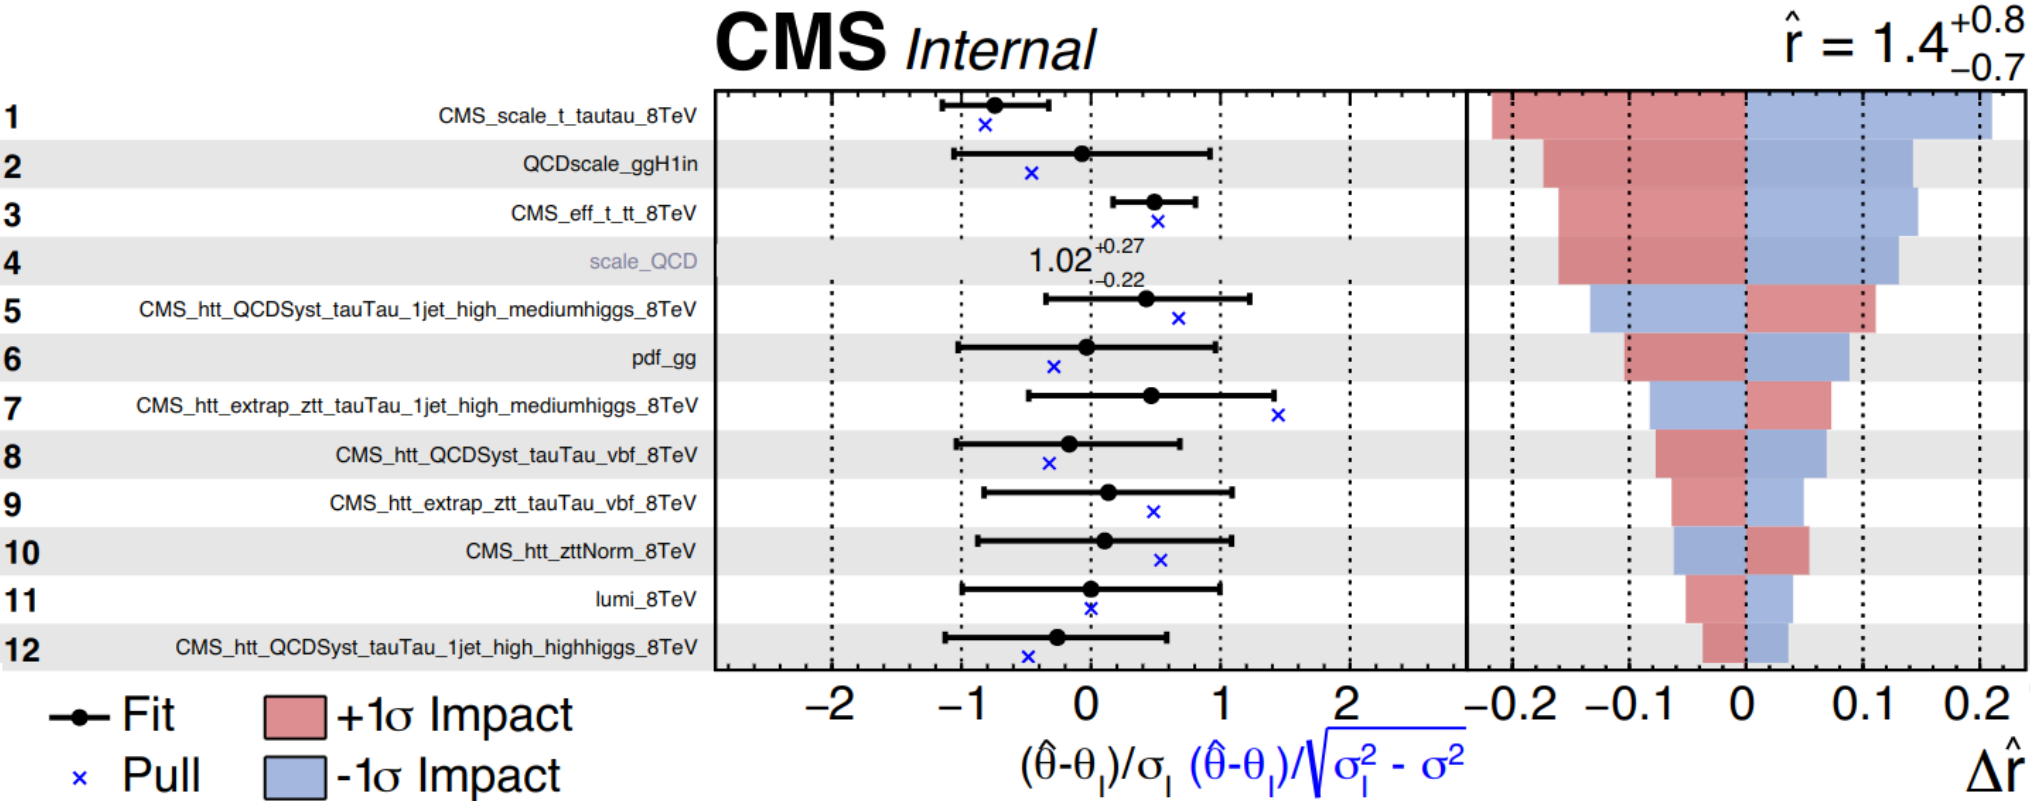
\includegraphics[width=1\linewidth]{fig/chap05-stats/impact.png}
    \caption{Example of an impact plot. In this plot, the POI $\mu$ is called $r$, and $\theta_I$, $\sigma_I$ are the pre-fit values.}
    \label{fig:impact}
\end{figure}


\subsection{Asimov dataset and sensitivity} The term $n_{cb}$ in \Eq{eq:likelihood} is the number of observed events in the b-th bin, so, it contains real data.\\
To perform a simulation of an analysis, $n_{cb}$ can be replaced by MC events, creating the so-called "Asimov dataset" \cite{Cowan2011AsymptoticPhysics}
\begin{equation}
    n_{cb}^{\text{Asimov}}=\sum_p y_{cpb}
\end{equation}
In this way will be always $\hat{\mu}=1$ and $\bm{\hat{\theta}}=0$.\\
Using the Asimov dataset, the statistical uncertainties on $\hat{\mu}$ can be estimated through an approximation.

\begin{enumerate}
    \item Let's consider the Poisson log-likelihood for a single bin
\begin{equation}
    \ln\left(\mathcal{L}_b(\mu)\right)=n_b \ln(\mu s_b + b_b) - (\mu s_b + b_b)-\ln n_b! 
\end{equation}
and let's find the maximum likelihood estimator for $\mu$
\begin{equation}
    \partial_\mu \ln{\mathcal{L}_b}=0 \implies \hat{\mu}=\frac{n_b-b_b}{s_b}
\end{equation}
The variance of the estimator $\hat{\mu}_b$ is
\begin{equation}
    {\mathrm{Var}}(\hat{\mu}_b)=\frac{{\mathrm{Var}}(n_b)}{s_b^2}=\frac{\mu s_b + b_b }{s_b^2}
\end{equation}
The variance of $\hat{\mu}_b$ depends on $\mu$ itself, but, in the context of the Asimov dataset, we can approximate it imposing $\mu=\hat{\mu}_b=1$, so the variance becomes
\begin{equation}
    {\mathrm{Var}}(\hat{\mu}_b)\sim \frac{s_b+b_b}{s_b^2}
\end{equation}
\newpage
 \item The Cramer-Rao theorem \cite{James2006StatisticalEdition} states that, for a probability density function of the exponential family, to whom the Poisson distribution belongs, it holds
\begin{equation}
    \mathrm{Var}(\hat{\mu})=-\frac{(1-\partial_\mu b)^2}{E[\partial_\mu^2 \ln \mathcal{L}]}
\end{equation}
where $b$ is the bias of the estimator.
The maximum likelihood estimator is asymptotically unbiased, so we can neglect $b$.
\begin{equation}
    E[\partial_\mu^2 \ln \mathcal{L}_b]\sim-\frac{1}{\mathrm{Var}(\hat{\mu}_b)}
\end{equation}
and for the total likelihood
\begin{equation}
    E[\partial_\mu^2 \ln \mathcal{L}]=
    \sum_b E[\partial_\mu^2 \ln \mathcal{L}_b]=\sum_b
    -\frac{1}{\mathrm{Var}(\hat{\mu}_b)}
\end{equation}
but since it holds $\mathrm{Var}(\hat{\mu}) =-1/E[\partial_\mu^2 \ln \mathcal{L}]$, then
\begin{equation}
    \mathrm{Var}(\hat{\mu})=\left[\sum_b \frac{1}{\mathrm{Var}(\hat{\mu}_b)}\right]^{-1}= \left[\sum_b \frac{s_b^2}{s_b+b_b} \right]^{-1}
\end{equation}
\end{enumerate}
So, to estimate the uncertainty on $\hat{\mu}$ using the Asimov dataset, we can compute the so-called \textbf{sensitivity}
\begin{equation}
    Q=\sum_c \sum_b \frac{s_{cb}^2}{s_{cb}+b_{cb}}
\end{equation}
and assert $\sigma(\hat{\mu}) \sim 1/\sqrt{Q}$\\
\\
Furthermore, the $(x_b,Q_b)$ plot helps us to choose the binning of the histogram to optimize the signal sensitivity.
